\documentclass[10pt,a4paper,oneside]{article}
\usepackage{cmap}
\usepackage[T2A]{fontenc}
\usepackage{float}
\usepackage{listings}
\usepackage{csquotes}
\usepackage[utf8]{inputenc}
\usepackage{amsmath}
\usepackage{amsfonts}
\usepackage{amssymb}
\usepackage[english, russian]{babel}%Подключаем русский язык.
\usepackage{graphicx}
\usepackage{geometry} % Меняем поля страницы.
\geometry{left=3cm} %Левое поле.
\geometry{right=2cm} %Правое поле.
\geometry{top=3cm} %Верхнее поле.
\geometry{bottom=2cm} %Нижнее поле.


%Начало документа
\begin{document}

%Создаём титульник.
\begin{titlepage}
\newpage
	%Название ВУЗа и институт.
	\begin{center}
		\Large Санкт-Петербургский Государственный Политехнический Университет\\
		Институт Компьютерных Наук и Технологий\\
	\end{center}
	%Кафедра.
	\begin{center}
		\large\textbf {Высшая школа интеллектуальных систем и суперкомпьютерных технологий}
	\end{center}
	
	%Пропуск места. 
	\vspace{5em}
	%!!!!!!!!!!!!!!!!!!!!!!!!!!!!!!!!!Название работы.
	\begin{center}
		\large{Отчёт по лабораторной работе №4 \\ на тему \\
		\textbf{Шум} }
	\end{center}
	
	%Делаем пропуск и пишем студента и преподавателя.
	\vspace{25em}
	\begin{flushright}
		\textbf{Работу выполнил\\}Студент группы 3530901/80203 \\ Танашкин В.А.\\
		\textbf{Преподаватель\\}Богач Н.В. 
	\end{flushright}
	
	\vspace{\fill}%В самом низу
	\begin{center}
	Санкт-Петербург, 2021 год	
	\end{center}
\end{titlepage} %Закончили титульный лист.

\section{Теоритическая часть о свойствах преобразования фурье}
Преобразование Фурье функции $f$ вещественной переменной является интегральным и задаётся следующими формулами: 
    
\[
    \begin{aligned}
        \text{Прямое: } && F(\nu) &= \int_{-\infty}^{\infty} f(t) e^{-2\pi i\nu t} dt \\
        \text{Обратное: } && f(t) &=  \int_{-\infty}^{\infty} F(\nu) e^{2\pi i\nu t} d\nu
    \end{aligned}
\]

\section{Свойства}
\subsection{Линейность}
    
По определению, для некоторого векторного пространства $(V,K,+,\cdot)$, $a,b \in V$, $\gamma \in K$:

\[
    \begin{aligned}
        f: V \rightarrow V \text{ - линейна}
        \Longleftrightarrow
        \begin{cases}
                \gamma\cdot f(a) = f(\gamma\cdot a) \\
                f(a) + f(b) = f(a + b)
        \end{cases}
    \end{aligned}
\]
    
Очевидно, что преобразование Фурье (ПФ) удовлетворяет этому условию (как функция на $(\mathbb{R} \rightarrow \mathbb{R},\mathbb{C},+,\cdot)$), а следовательно:

\[
    \begin{aligned}
        Fourier\left(\sum_{i}\alpha_i\phi_i(t)\right)
        &= \sum_{i}\alpha_i \cdot Fourier(\phi_i(t)) \\
        &= \sum_{i}\alpha_i \Phi_i(\nu)
    \end{aligned}
\]

\subsection{Смещение функции}

При смещении функции $\phi(t)$ на $\Delta t$ результат ПФ умножается на $e^{2\pi i \nu\Delta t}$. Пусть $t' = t + \Delta t$, тогда:

\[
    \begin{aligned}
        Fourier\left(\phi(t + \Delta t)\right)
        &= \int_{-\infty}^{\infty} \phi(t + \Delta t) e^{-2\pi i\nu t} dt \\
        &= \int_{-\infty}^{\infty} \phi(t') e^{-2\pi i\nu (t' - \Delta t)} dt
    \end{aligned}
\]

Так как $dt' = d(t + \Delta t) = dt$, то:

\[
    \begin{aligned}
        \int_{-\infty}^{\infty} \phi(t') e^{-2\pi i\nu (t' - \Delta t)} dt'
        &= e^{2\pi i\nu\Delta t} \cdot \int_{-\infty}^{\infty} \phi(t') e^{-2\pi i\nu t'} dt' \\
        &= e^{2\pi i\nu\Delta t} \cdot F(\nu)
    \end{aligned}
\]

\subsection{Масштабирование функции}

Пусть $t' = \alpha t$, тогда:

\[
    \begin{aligned}
        Fourier\left(\phi(\alpha t)\right)
        &= \int_{-\infty}^{\infty} \phi(\alpha t) e^{-2\pi i\nu t} dt \\
        &= \int_{-\infty}^{\infty} \phi(t') e^{-2\pi i\nu \frac{t'}{\alpha}} dt
    \end{aligned}
\]

Так как $dt' = \alpha dt$, то для $a > 0$:

\[
    \begin{aligned}
        \int_{-\infty}^{\infty} \phi(t') e^{-2\pi i\nu \frac{t'}{\alpha}} dt
        &= \frac{1}{\alpha} \int_{-\infty}^{\infty} \phi(t') e^{-2\pi i\frac{\nu}{\alpha} t'} dt \\
        &= \frac{1}{\alpha} \Phi\left(\frac{\nu}{\alpha}\right)
    \end{aligned}
\]

Для $a < 0$ получится $dt' < 0$ при $dt > 0$. При этом нужно поменять пределы интегрирования местами, тогда получим результат с отрицательным знаком:

\[
    \begin{aligned}
        -\frac{1}{\alpha} \Phi\left(\frac{\nu}{\alpha}\right)
    \end{aligned}
\]

Таким образом, в одной форме это:

\[
    \begin{aligned}
        \frac{1}{\left|\alpha\right|} \Phi\left(\frac{\nu}{\alpha}\right)
    \end{aligned}
\]

Вывод: при сжатии функции по времени в $\alpha$ раз, её ПФ расширяется по частоте в $\alpha$ раз.

\subsection{Перемножение функции}

ПФ произведения двух функций - это свёртка их ПФ.

\[
    \begin{aligned}
        Fourier\left(\phi(t)\xi(t)\right) 
        &= \int_{-\infty}^{\infty} \phi(t)\xi(t) e^{-2\pi i\nu t} dt \\
        &= \int_{-\infty}^{\infty} \left( \int_{-\infty}^{\infty} \Phi(k) e^{2\pi i kt} dk \right) \xi(t) e^{-2\pi i\nu t} dt \\
        &= \int_{-\infty}^{\infty} \Phi(k) \left( \int_{-\infty}^{\infty} \xi(t) e^{2\pi i (k - \nu)t} dt \right) dk \\
        &= \int_{-\infty}^{\infty} \Phi(k) \left( \int_{-\infty}^{\infty} \xi(t) e^{-2\pi i (\nu - k)t} dt \right) dk \\
        &= \int_{-\infty}^{\infty} \Phi(k) \Xi(\nu - k) dk \\
        &= \left(\Phi * \Xi\right)(\nu)
    \end{aligned}
\]

\subsection{Свёртывание функции}

ПФ свёртки двух функций есть произведение ПФ этих функций. Доказывается аналогично в силу \textquote{симметрии} прямого и обратного преобразований Фурье.

\subsection{Дифференцирование функции}

При дифференцировании $\phi(t)$ по $t$ её ПФ умножается на $2\pi i \nu$.

\[
    \begin{aligned}
        Fourier\left(\frac{d\phi(t)}{dt}\right) 
        &= \int_{-\infty}^{\infty} \frac{d\phi(t)}{dt} e^{-2\pi i\nu t} dt \\
        &= \int_{-\infty}^{\infty} e^{-2\pi i\nu t} d\phi(t) \\
        &= \phi(t) e^{-2\pi\nu t} \bigg|_{-\infty}^{\infty} - \int_{-\infty}^{\infty} \phi(t) d\left(e^{-2\pi i\nu t}\right) \\
        &= \phi(t) e^{-2\pi\nu t} \bigg|_{-\infty}^{\infty} + 2\pi i\nu \int_{-\infty}^{\infty} \phi(t) e^{-2\pi i\nu t} dt \\
        &= \phi(t) e^{-2\pi\nu t} \bigg|_{-\infty}^{\infty} + 2\pi i\nu \cdot \Phi(\nu) \\
    \end{aligned}
\]

Прямое и обратное преобразование Фурье существует для функций с ограниченной энергией, то есть:

\[
    \begin{aligned}
        \int_{-\infty}^{\infty} |\phi(t)|^2 dt \neq \infty
    \end{aligned}
\]

И из этого следует, что первое слагаемое равно 0.

\subsection{Интегрирование функции}

При интегрировании ПФ делится на $2\pi i \nu$.

\[
    \begin{aligned}
        Fourier\left(\int_{-\infty}^{t} \phi(t') dt'\right) 
        &= \int_{-\infty}^{\infty} \left( \int_{-\infty}^{t} \phi(t') dt' \right) e^{-2\pi i\nu t} dt \\
        &= -\frac{1}{2\pi i\nu} \cdot \int_{-\infty}^{\infty} \left( \int_{-\infty}^{t} \phi(t') dt' \right) d\left(e^{-2\pi i\nu t}\right) \\
        &= -\frac{1}{2\pi i\nu} \cdot \left[ e^{-2\pi i\nu t} \int_{-\infty}^{t} \phi(t') dt' \biggr|_{-\infty}^{\infty} - \int_{-\infty}^{\infty} e^{-2\pi i\nu t} d\left(\int_{-\infty}^{t} \phi(t') dt'\right)\right] \\
        &= -\frac{1}{2\pi i\nu} \cdot \left[ e^{-2\pi i\nu t} \int_{-\infty}^{t} \phi(t) dt \biggr|_{-\infty}^{\infty} - \int_{-\infty}^{\infty} e^{-2\pi i\nu t} \phi(t) dt\right] \\
        &= -\frac{1}{2\pi i\nu} \cdot \left[ 0 - \int_{-\infty}^{\infty} e^{-2\pi i\nu t} \phi(t) dt\right] \\
        &= \frac{1}{2\pi i\nu} \cdot \int_{-\infty}^{\infty} e^{-2\pi i\nu t} \phi(t) dt \\
        &= \frac{1}{2\pi i\nu} \cdot \Phi(\nu)
    \end{aligned}
\]

0 возникает потому, что $\int_{-\infty}^{\infty} \phi(t') dt' = 0$.

\subsection{Обратимость}

Преобразования обратимы, причём обратное преобразование имеет практически такую же форму, как и прямое преобразование.


\section{Упражнение номер №1}

Необходимо скачать звук природных источников шума. Определить похож ли спектр мощности скаченного звука на белый розовый или броуновский шумы.

Для данного задания я взял звук волн черного моря из репозитория и выбрал небольшой сегмент 5 секунда длительность 1с

Распечатаем спектр: 

\begin{figure}[H]
        \centering
        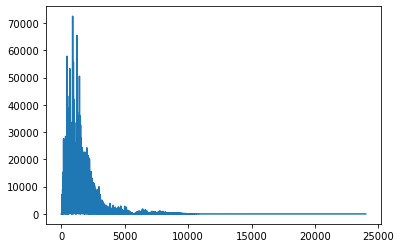
\includegraphics[width=0.75\textwidth]{1.png}
        \caption{2}
        \label{fig:first}
\end{figure}

Амплитуда падает с частотой, поэтому это может быть красный или розовый шум. Мы можем проверить это, посмотрев на спектр мощности в логарифмической шкале.

\begin{figure}[H]
        \centering
        \includegraphics[width=0.75\textwidth]2.png}
        \caption{2}
        \label{fig:first}
\end{figure}

Амплитуда этой структуры сначала увеличивается, а затем уменьшается. Это обычное явлением для естественных источников шума. Выберем другой отрезок (начало: 10сек и длительность 1 сек) и вывдедем спектр для сравнения:


\begin{figure}[H]
        \centering
        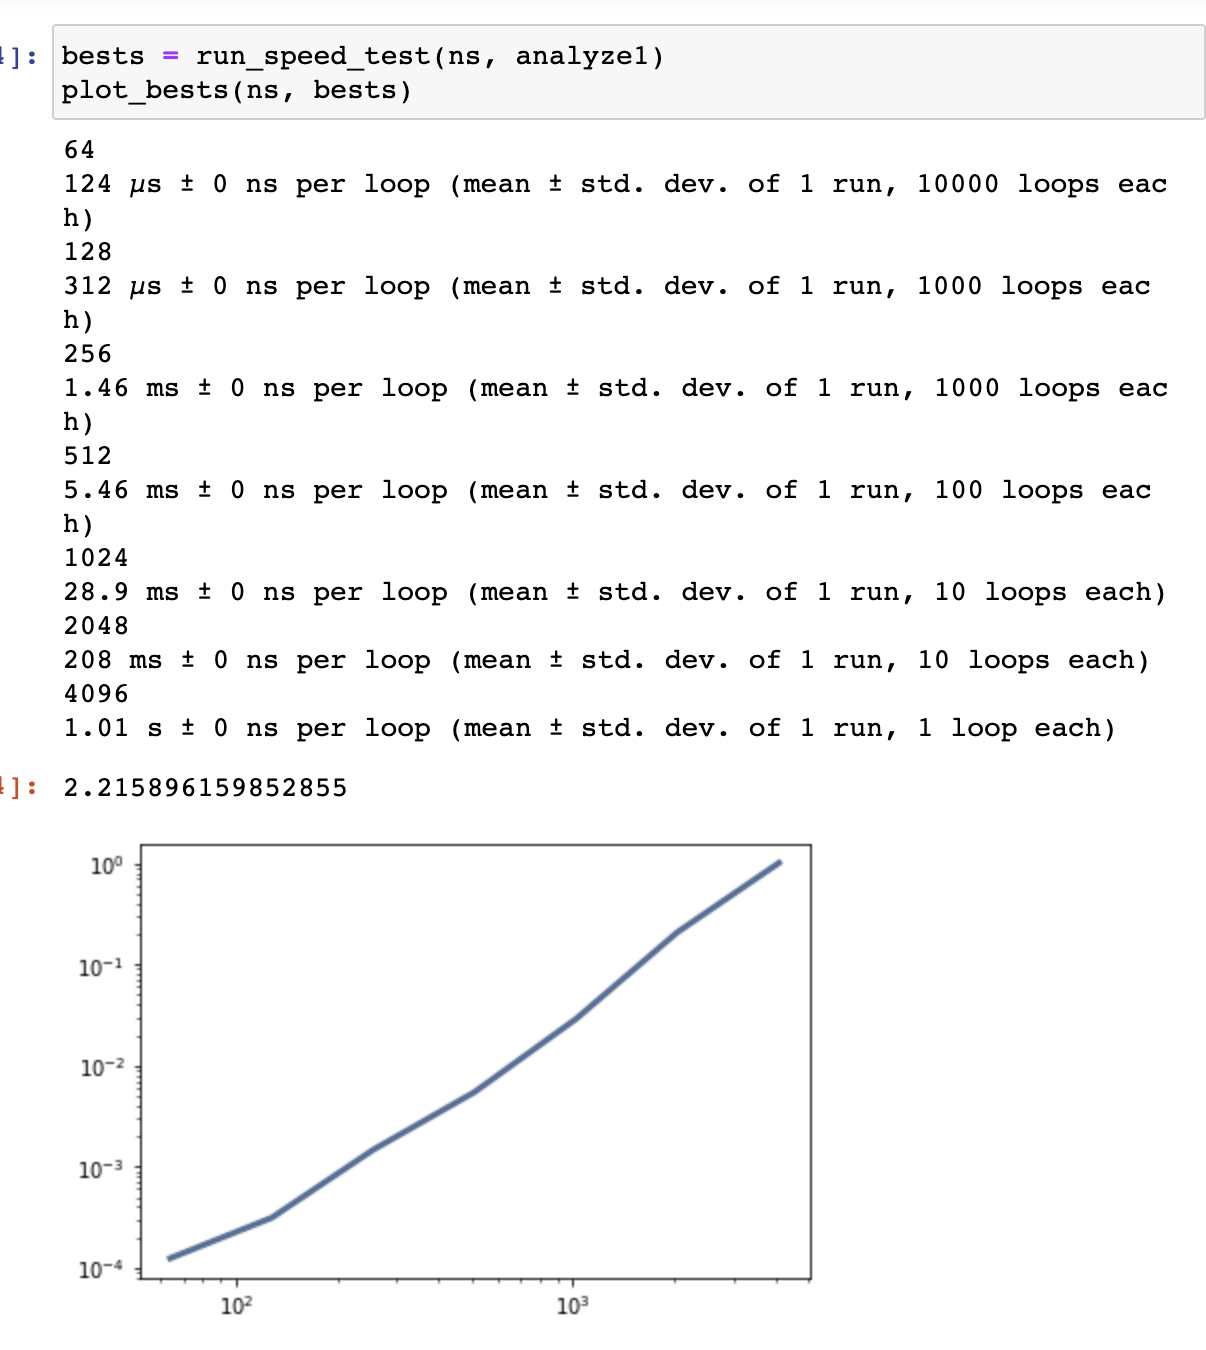
\includegraphics[width=0.75\textwidth]{3.png}
        \caption{2}
        \label{fig:first}
\end{figure}

Рассмотрим их в логарифмической метрики:

\begin{figure}[H]
        \centering
        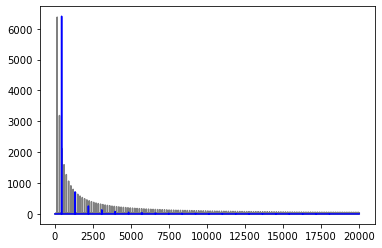
\includegraphics[width=0.75\textwidth]{4.png}
        \caption{2}
        \label{fig:first}
\end{figure}

Из данного сравнения мы можем заметить что поведение данной структуры остается практически неизменным с течением времени.

\begin{figure}[H]
        \centering
        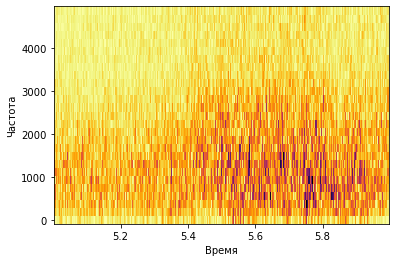
\includegraphics[width=0.75\textwidth]{5.png}
        \caption{2}
        \label{fig:first}
\end{figure}

В этом сегменте общая амплитуда падает, но смесь частот кажется стабильной.

\section{Упражнение номер №2}

Реализовать метод Бартлетта и с помощью него провести оценку спектра мощности шумового сигнала.

bartlett_method создает спектрограмму и извлекает spec_map, который отображает время на объекты Spectrum. Он вычисляет PSD для каждого спектра, складывает их и помещает результаты в объект Spectrum.

Реализуем метод и построим график: 

\begin{figure}[H]
        \centering
        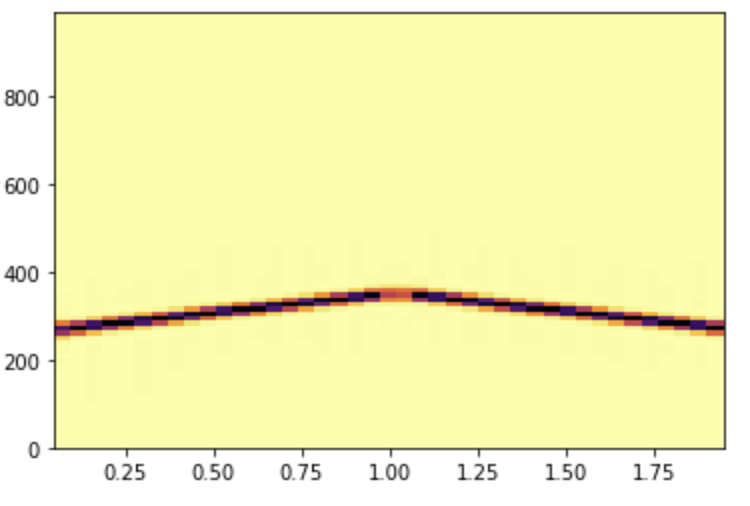
\includegraphics[width=0.75\textwidth]{6.png}
        \caption{2}
        \label{fig:first}
\end{figure}

Теперь мы можем более четко увидеть взаимосвязь между мощностью и частотой. Это не простая линейная зависимость, более того, она одинакова для разных сегментов, даже в деталях, таких как выемки около 1000 Гц, 4000 Гц и тд..


\section{Упражнение номер №3}

Открыть файл об исторических данных о ежедневной цене биткоина. Вычислить спектр цен на биткоин как функцию времени. Определить схожесть с  белым розовым или броуновским шумами.

Выгрузка даты об изменении цены на биткоин в долларх в период с 1 января 2020 по 1 января 2021

Построим график: 

\begin{figure}[H]
        \centering
        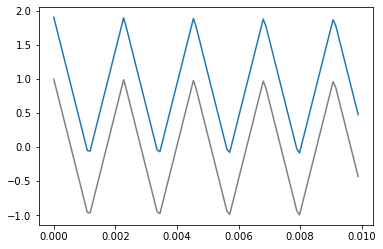
\includegraphics[width=0.75\textwidth]{7.png}
        \caption{2}
        \label{fig:first}
\end{figure}

Построим спектр, где частотa ~ 1/дни:

\begin{figure}[H]
        \centering
        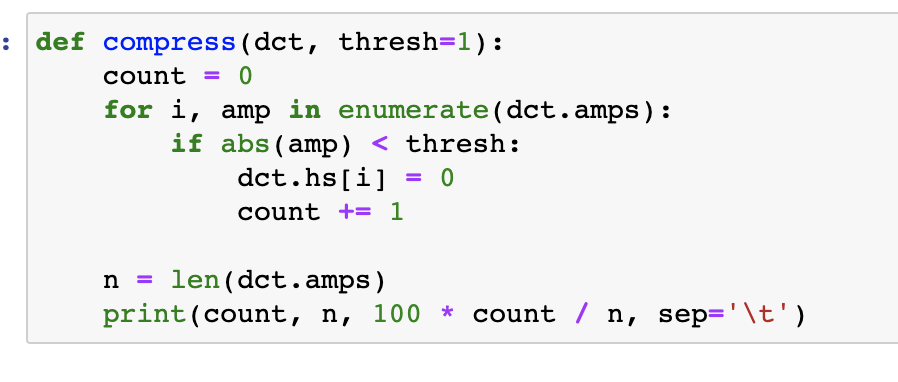
\includegraphics[width=0.75\textwidth]{8.png}
        \caption{2}
        \label{fig:first}
\end{figure}

Красный шум должен иметь наклон -2. Наклон этого спектра близок к -1,7, сложно сделать вывод о принадлежности его к розовому или красному шумам.

\section{Упражнение номер №4}

Необходимо реалищовать класс, UncorrelatedPoissonNoise, который наследуется от _Noise и обеспечивает оценку. Он должен использовать np.random.poisson для генерации случайных значений из распределения Пуассона. Параметр этой функции lam - среднее количество частиц за каждый интервал. Для этого мы можем использовать атрибут amp, чтобы указать lam. Например, если частота кадров составляет 10 кГц, а ампер - 0,0005, мы ожидаем около 5 «щелчков» в секунду.

Реализуем класс: 

\begin{figure}[H]
        \centering
        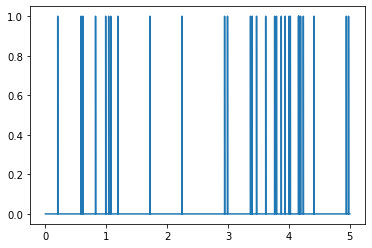
\includegraphics[width=0.75\textwidth]{9.png}
        \caption{2}
        \label{fig:first}
\end{figure}

Прослушаем этот звук
\end{figure}

Чтобы убедиться, что все работает, мы сравниваем ожидаемое количество частиц и фактическое количество:

Ожидаем: 25, фактически: 31

Рассмотрим волну и также рассмотрим спектр мощности в логарифмической метрики:

\begin{figure}[H]
        \centering
        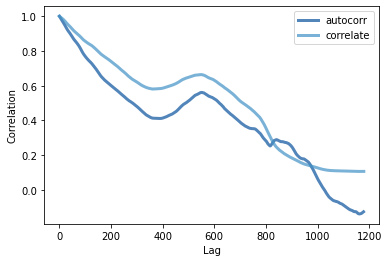
\includegraphics[width=0.75\textwidth]{10.png}
        \caption{2}
        \label{fig:first}
\end{figure}

Наклон составляет -0.0051, что практически соотвестувует белому шуму.

Выведем звук при высоком уровне радиации и отобразим волну на графике: 

\begin{figure}[H]
        \centering
        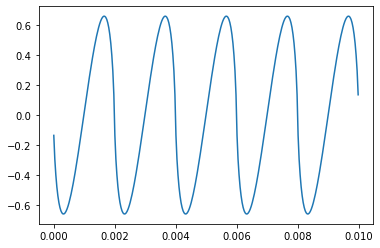
\includegraphics[width=0.75\textwidth]{11.png}
        \caption{2}
        \label{fig:first}
\end{figure}

И спектр сходится на гауссовском шуме.

\begin{figure}[H]
        \centering
        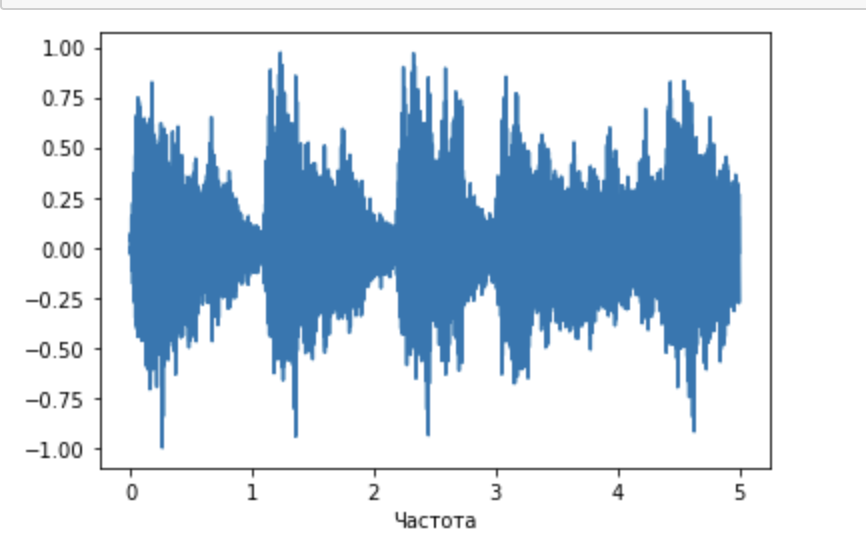
\includegraphics[width=0.75\textwidth]{12.png}
        \caption{2}
        \label{fig:first}
\end{figure}


\section{Упражнение номер №5}

Изучить способ более эффективного варианта реализации алгоритма для генерации розового шума. Вычислить спектр результата и убедиться, что соотношение между мощностью и частотой соответствующее. 

Используем алгоритм Восса-Маккартни.


Построим волну: 

\begin{figure}[H]
        \centering
        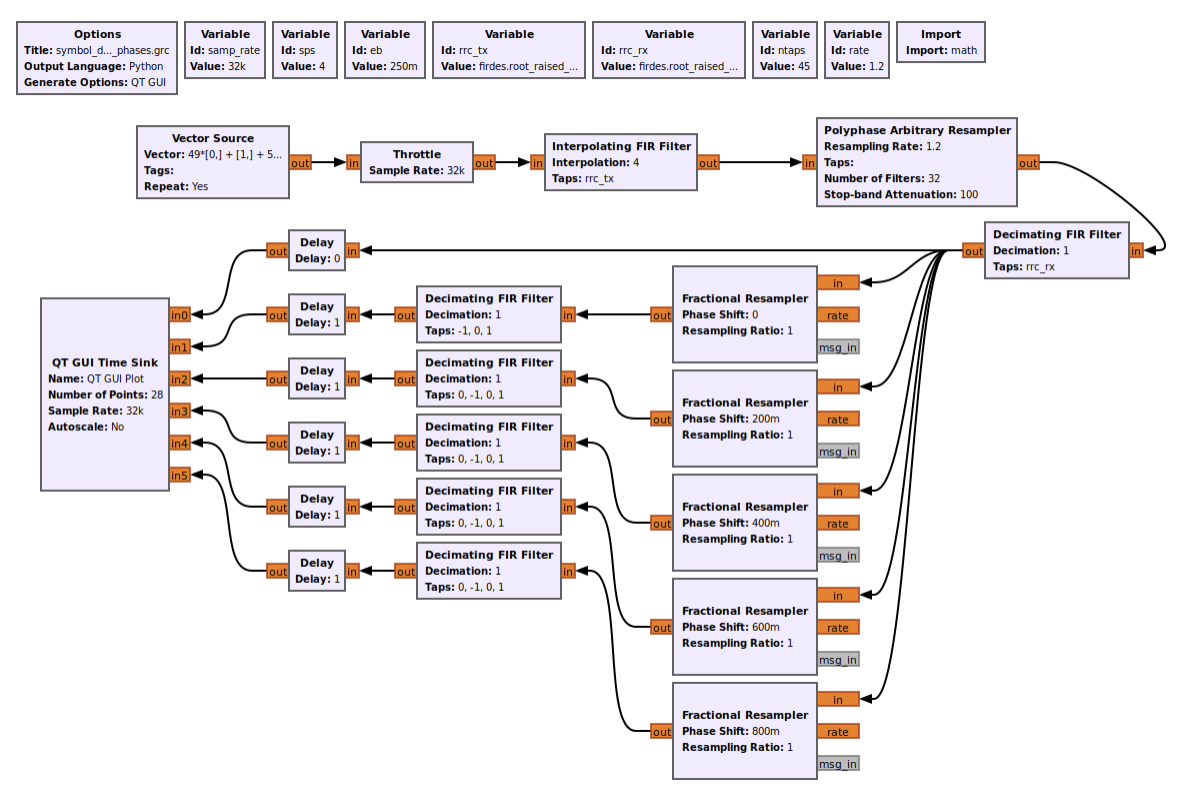
\includegraphics[width=0.75\textwidth]{13.png}
        \caption{2}
        \label{fig:first}
\end{figure}

Можем прослушать данный сигнал и вычислить спектр мощности: 

\begin{figure}[H]
        \centering
        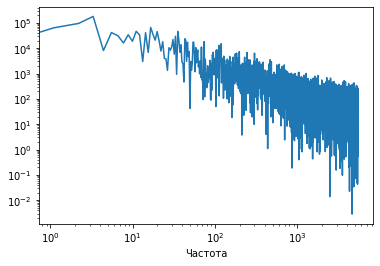
\includegraphics[width=0.75\textwidth]{14.png}
        \caption{2}
        \label{fig:first}
\end{figure}

Вычислив наклон мы видим что он близок к -1 (примерно -0.98). Для более лучшего понимания среднего спектра мощности мы должны сгенерировать более длинную выборку

\begin{figure}[H]
        \centering
        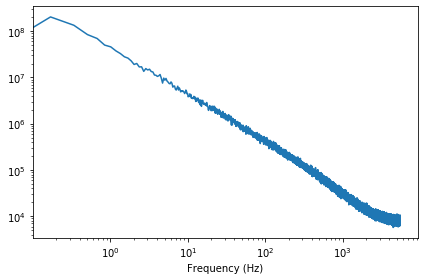
\includegraphics[width=0.75\textwidth]{15.png}
        \caption{2}
        \label{fig:first}
\end{figure}

Это довольно близко к прямой линии с некоторой кривизной на самых высоких частотах. Наклон близок к -1

\end{document}
